%% LyX 2.1.4 created this file.  For more info, see http://www.lyx.org/.
%% Do not edit unless you really know what you are doing.
\documentclass[english]{article}
\usepackage[T1]{fontenc}
\usepackage[latin9]{inputenc}
\usepackage{geometry}
\geometry{verbose,tmargin=2cm,bmargin=3cm,lmargin=1.5cm,rmargin=1.5cm}
\usepackage{mathtools}
\usepackage{amsmath}
\usepackage{amssymb}
\usepackage{graphicx}

\makeatletter

%%%%%%%%%%%%%%%%%%%%%%%%%%%%%% LyX specific LaTeX commands.
%% Because html converters don't know tabularnewline
\providecommand{\tabularnewline}{\\}

%%%%%%%%%%%%%%%%%%%%%%%%%%%%%% User specified LaTeX commands.
\usepackage{tikz}
\usepackage{babel}
\renewcommand{\labelitemi}{$\diamond$}
\newcommand{\T}{\rule{0pt}{2.6ex}}       % Top strut
\newcommand{\B}{\rule[-1.2ex]{0pt}{0pt}} % Bottom strut






\makeatother

\usepackage{babel}
\begin{document}

\title{COMP8620: MC-AIXI-CTW\\
Group 3}


\author{Jarryd Martin, John Aslanides, Yadunandan Sannappa,\\
 Nrupendra Rao, Cheng Yu, Ryk Budzynski}


\date{October 2015}

\maketitle
We outline an implementation of Veness et al.'s Monte Carlo AIXI approximation\cite{veness-11},
and report our simulation results on a number of toy domains.


\section{Introduction}

Recall that the AIXI agent is defined by its actions, which for each
cycle $k$ are given by 
\[
a_{k}^{\text{AIXI}}=\arg\max_{a_{k}}\sum_{o_{k}r_{k}}\cdots\max_{a_{m}}\sum_{o_{m}r_{m}}\left[r_{k}+\dots+r_{m}\right]\xi\left(o_{1}r_{1}\dots o_{m}r_{m}|a_{1}\dots a_{m}\right),
\]


where the $o_{n}$ and $r_{n}$ are the observation and reward provided
by the environment at cycle $n$, and $\xi$ is a Bayesian mixture
model for the environment. 

Following Veness et al., we approximate $a_{k}^{\text{AIXI}}$ using
Monte Carlo tree search (upper confidence bound) to approximate the
expectimax, we compute a mixture over variable-order Markov models
using the context-tree weighting algorithm. This approximation is
denoted MC-AIXI-CTW.

We present a lightweight C++ implementation of MC-AIXI-CTW, along
with implementations of a number of simple games: $\textsc{Pacman},\ $
$\textsc{Tic-Tac-Toe}$, $\textsc{Biased Rock-Paper-Scissor}$, $\textsc{Extended-Tiger}$,
and $\textsc{Cheesemaze}$.


\subsection{Files}

The report archive should contain the following: 
\begin{verbatim}

MC-AIXI-CTW-Grp3.zip
    \report
        report.pdf // this report
        report.tex
        cheesemaze_01.png // results plots
        extended_tiger_01.png
        biased_rock_paper_scissor_01.png
        tic_tac_toe_01.png
        pacman_01.png
    \src
        main.hpp
        main.cpp
        environment.hpp
        environment.cpp
        agent.hpp
        agent.cpp
        search.hpp
        search.cpp
        predict.hpp
        predict.cpp
        util.hpp
        util.cpp
        README.md
        cheesemaze.conf // environment configuration files
        rockpaper.conf
        tictactoe.conf
        coinflip.conf
        tiger.conf

        
\end{verbatim}

\subsection{User Manual}


\section{MC-AIXI-CTW Implementation}


\subsection{Monte Carlo Tree Search (MCTS) Algorithm}
\begin{enumerate}
\item Source code files 
\item Class structure (SearchNode, DecisionNode, ChanceNode, ...) 
\item Description of the algorithm (Veness...) 
\end{enumerate}

\subsection{Context Tree Weighting (CTW)}


\subsection{Environments}


\subsubsection{Cheesemaze}


\subsubsection{Extended Tiger}


\subsubsection{Biased Rock-Paper-Scissor}


\subsubsection{Tic-Tac-Toe}


\subsubsection{Pacman}


\section{Simulation Results}


\subsection{Cheesemaze}
\begin{itemize}
\item Experimental setup ... \\
 Any simulation provided should include detailed description of experimental
setup; selected parameters of algorithms and examples; and concise
interpretations of obtained simulation results. \\



\begin{tabular}{|l|l|l|c}
\hline 
Environment  & MCTS  & CTW  & \tabularnewline
\hline 
1  & $m=100$  & $\text{ct-depth}=96$  & \tabularnewline
\hline 
 & $C=\sqrt{2}$  &  & \tabularnewline
\hline 
\end{tabular}

\item Plots ... \\
 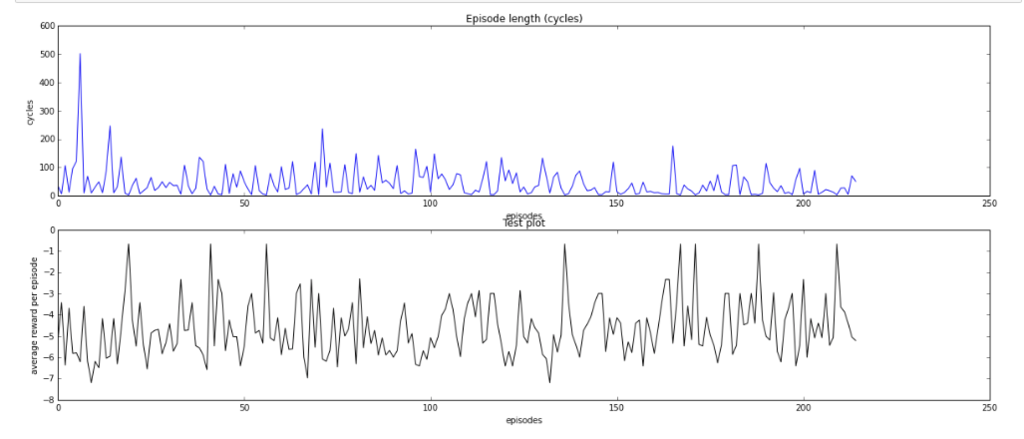
\includegraphics[scale=0.4]{cheesemaze_01} 
\item Interpretation of Results 
\end{itemize}

\subsection{Extended Tiger}

Experimental setup ... \\
 Plots ... 


\subsection{Biased Rock-Paper-Scissor}

Experimental setup ... \\
 Plots ... 


\subsection{Tic-Tac-Toe}

Experimental setup ... \\
 Plots ... 


\subsection{Pacman}

Experimental setup ... \\
 Plots ... 


\section{Cross Domain Simulation Results}

Cheesemaze and Extended Tiger


\section{Possible Other things}

Cross domain simulation on more difficult environments... \\
 Separate CTW for Obs and Rews...

 \bibliographystyle{unsrt}
\bibliography{report}

\end{document}
